\newpage

\thispagestyle{empty}

\pagenumbering{roman} 

\setcounter{page}{1}

\begin{center}
\includegraphics[clip,width=4cm,keepaspectratio]{Figures/TUM_Logo}\par\end{center}

\begin{center}\vspace*{1.5cm} {\Large Lehrstuhl für \\ Elektrische Antriebssysteme \& Leistungselektronik}{\large }\\
{\large Technische Universität München}\\
{\large Professor Dr.-Ing. Ralph Kennel}\par\end{center}{\large \par}

\vspace*{1.0cm}

\begin{center}{\large <Bearbeiter>}\par\end{center}{\large \par}

\begin{center}\vspace*{1.0cm}\par\end{center}

\begin{center}{\huge <Titel der Arbeit>}\par\end{center}{\huge \par}

\begin{center}\vspace*{1.5cm}\par\end{center}

\begin{center}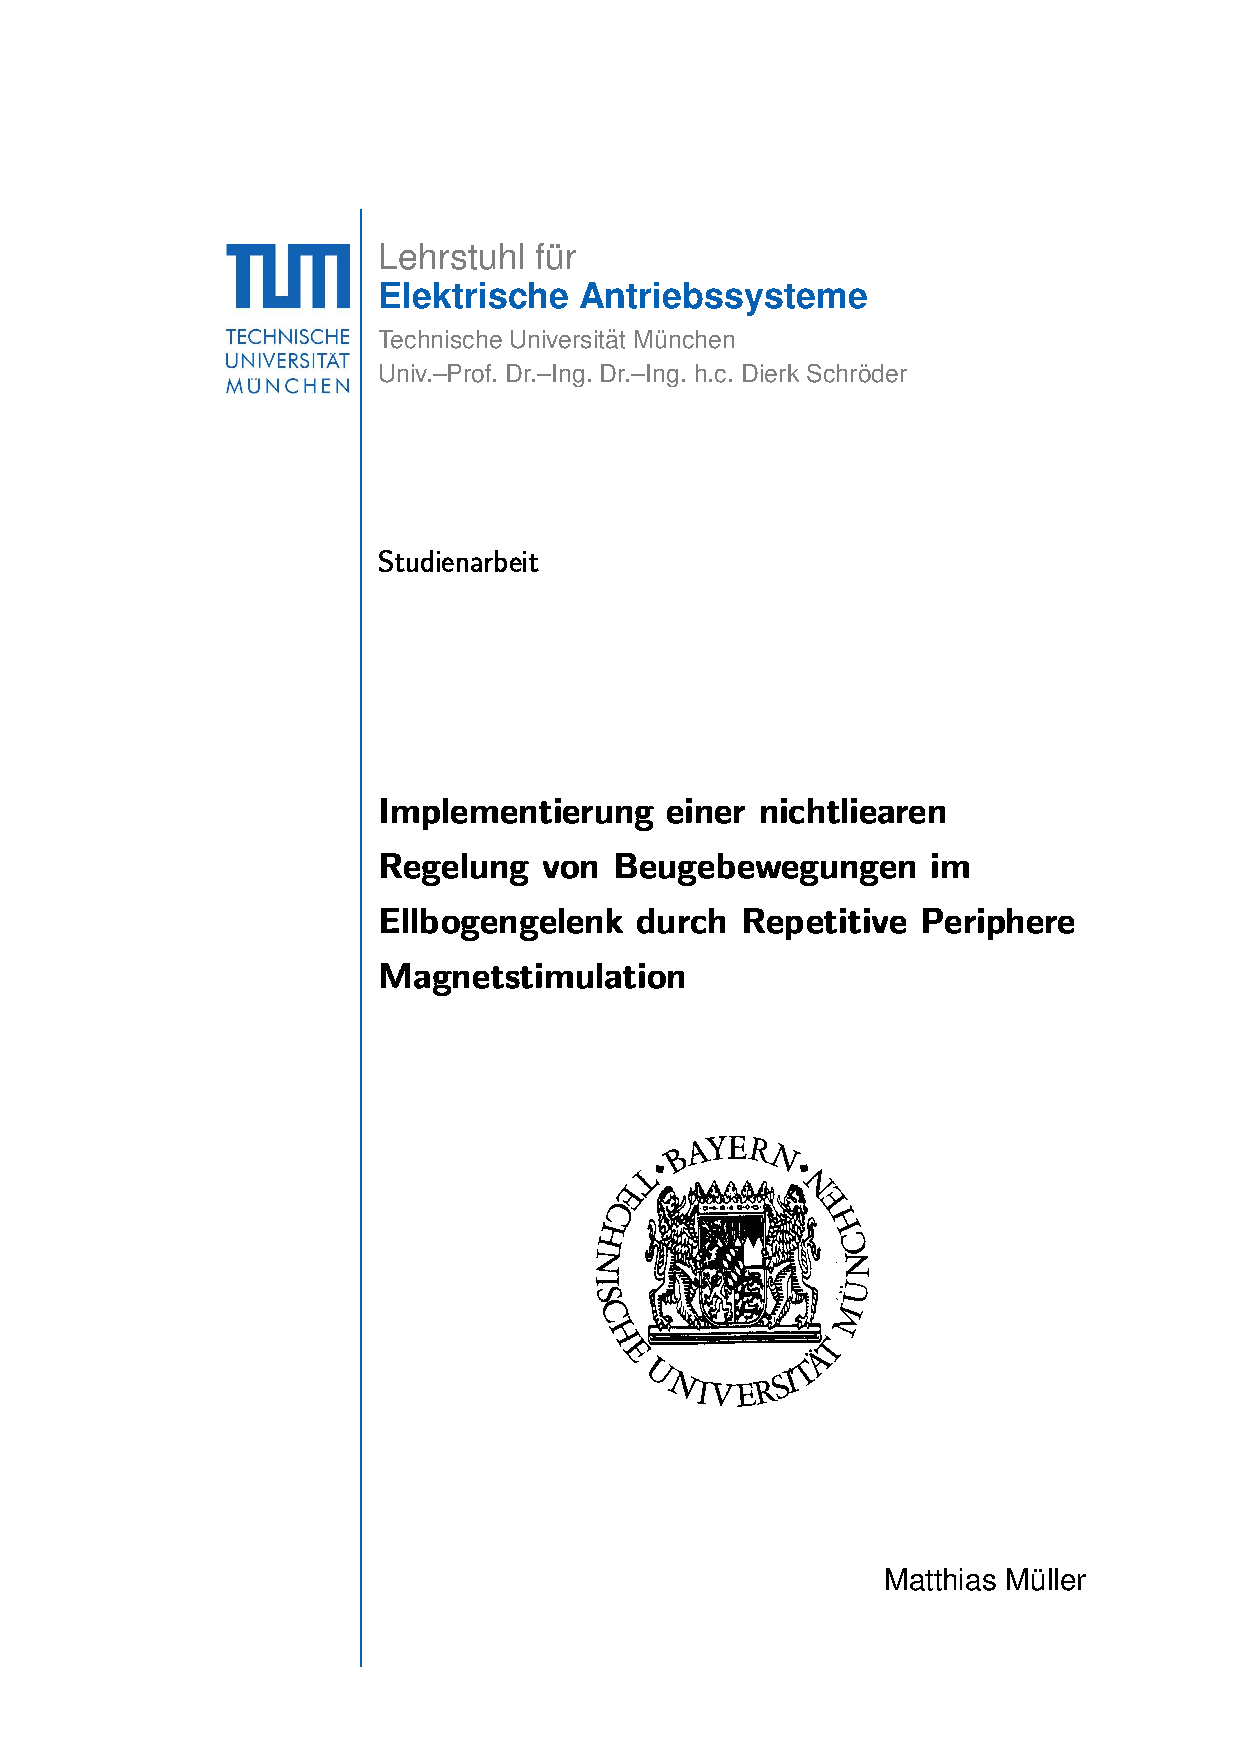
\includegraphics[clip,width=5.5cm,keepaspectratio]{Figures/TUM_Wappen}\par\end{center}

\newpage

\mbox{}

\thispagestyle{empty}

\newpage

\thispagestyle{empty}

\begin{center}\begin{tabular}{c}
{\Large Lehrstuhl für}  \tabularnewline
{\Large Elektrische Antriebssysteme \& Leistungselektronik} \tabularnewline
{\large Technische Universität München}\tabularnewline
{\large Professor Dr.-Ing. Ralph Kennel}\tabularnewline
{\small Arcisstraße 21, 80333 München}\tabularnewline
{\scriptsize Tel.: 089/289 28358\hspace{1cm} ~Fax: 089/289 28336
\hspace{1cm} ~email: eat@ei.tum.de}\tabularnewline
\hline
\end{tabular}\par\end{center}

\begin{center}\vspace*{2.0cm} \par\end{center}

\begin{center}{\large <Bearbeiter>}\par\end{center}{\large \par}

\vspace*{1.0cm}

\begin{center}{\huge <Titel der Arbeit>}\par\end{center}{\huge \par}

\begin{center}\newpage

\mbox{}

\thispagestyle{empty}\par\end{center}

\newpage

\thispagestyle{empty}

\begin{center}{\LARGE <Titel der Arbeit>}\par\end{center}{\LARGE \par}

\vspace{1.5cm}

\begin{center}Lehrstuhl für \\ Elektrische Antriebssysteme \& Leistungselektronik\\
der Technischen Universität München\\
Professor Dr.-Ing. Ralph Kennel\par\end{center}

\hfill

\begin{center}Submitted for the Degree of <Bachelor/Master> of Science <(B.Sc./M.Sc.)> \\ 
in Electrical Engineering and Information Technology (TUM) \par\end{center}

\vspace{0.8cm}

\begin{center}{\large <Bearbeiter>}\par\end{center}{\large \par}

\vspace{1.0cm}

\begin{center}Born <Geburtsdatum> in <City, Country>\par\end{center}

\vspace{1cm}

\begin{center}<Street \#?>\\
<Zip Code, City>\par\end{center}

\vspace{1cm}

\hspace*{-4cm}

\begin{flushleft}\begin{tabular}{ll}
Supervision\hfill :&
<Dipl.-Ing. Christoph Hackl>\tabularnewline
&
\tabularnewline
Beginning \hfill :&
??.??.????\tabularnewline
End\hfill :&
??.??.????\tabularnewline
Date of Presentation\hfill ~:&
??.??.????\tabularnewline
\end{tabular}\par\end{flushleft}

\newpage

\mbox{}

\thispagestyle{empty}


\chapter*{Acknowledgement}

\addcontentsline{toc}{chapter}{\numberline{}{Acknowledgement}} <blabla>
\\


\begin{flushright}<Bearbeiter>\par\end{flushright}

\newpage \thispagestyle{empty} \addcontentsline{toc}{chapter}{\numberline{}{Problem
Statement}}

\vspace*{-1cm}
\begin{center}\begin{tabular}{c}
{\Large Lehrstuhl für}  \tabularnewline
{\Large Elektrische Antriebssysteme \& Leistungselektronik} \tabularnewline
{\large Technische Universität München}\tabularnewline
{\large Professor Dr.-Ing. Ralph Kennel}\tabularnewline
{\small Arcisstraße 21, 80333 München}\tabularnewline
{\scriptsize Tel.: 089/289 28358\hspace{1cm} ~Fax: 089/289 28336
\hspace{1cm} ~email: eat@ei.tum.de}\tabularnewline
\hline
\end{tabular}\par\end{center}

\begin{center}\vspace{0.5cm}\par\end{center}

\begin{center}{\Large <BACHELORTHESIS/MASTERTHESIS> \# <BA/MA Nummer (in
Sekretariat erfragen)>}\par\end{center}{\Large \par}

\begin{center}\vspace{0.5cm} \begin{tabular}{cl}
Name of Student\hfill:&
\multicolumn{1}{l}{<Vorname Name>}\tabularnewline
&
 <Strasse>\tabularnewline
&
<Postleitzahl Ort>\tabularnewline
&
\tabularnewline
Interest of Study\hfill:&
Elektrotechnik \& Informationstechnik \tabularnewline
&
Schwerpunkte <?>\tabularnewline
&
\tabularnewline
Title of Thesis\hfill:&
<Titel der Arbeit>\tabularnewline
&
\tabularnewline
&
\tabularnewline
Supervisor\hfill:&
<Dipl.-Ing. Christoph Hackl>\tabularnewline
&
\tabularnewline
&
\tabularnewline
\multicolumn{2}{l}{Problem Statement}\tabularnewline
\end{tabular}\par\end{center}

\begin{enumerate}
\item Task 1...
\item {\small safasf}{\small \par}
\item {\small safasf}{\small \par}
\end{enumerate}
\hfill\begin{tabular}{c}
\hfill\tabularnewline
\hline
Prof. Dr.-Ing. Ralph Kennel\tabularnewline
\end{tabular}


\chapter*{Declaration}

\addcontentsline{toc}{chapter}{\numberline{}{Declaration}} The work
in this thesis is based on research carried out at the Institute for
Electrical Drive Systems and Power Electronics, Technische Universität München (TUM) supervised
by <Dipl.-Ing. Christoph Hackl>. No part of this thesis has been submitted
elsewhere for any other degree or qualification and it is all my own
work unless referenced to the contrary in the text.\vspace{2in}

\vfill{}
\noindent \textbf{Copyright} $\mathbf{\copyright}$ \textbf{<Jahr>
by <Bearbeiter>.}\\
 {}``The copyright of this thesis rests with the author. No quotations
from it should be published without the author's prior written consent
and information derived from it should be acknowledged''.

\newpage

\mbox{}

\thispagestyle{empty}

\selectlanguage{english}

\tableofcontents{}

\newpage

\mbox{}

\thispagestyle{empty}

\listoffigures


\newpage

\mbox{}

\thispagestyle{empty}

\listoftables

